\chapter{Vorlesung}
\section*{Heapsort (Fortsetzung)}

\section{Pseudocode}
\begin{lstlisting}
heapify ( int[] a, int i, int n) {
  while (2i + 1 < n) {		//linkes Kind von i existiert
    int j = 2i + 1;
    if ( 2i +2 < n)  		//rechtes Kind von i existiert
      if ( a[j] < a[j+1])
        j = j + 1;  		//j steht für Indes des größten Kindes
    if ( a[i] > a[j])  		//Vater größer als Kind
      break;  			//Abbruch, weil heap bereits erfüllt
    swap(a,i,j); 		//Tausch zwischen Vater und Kind
    i = j;
  }
}
\end{lstlisting}
\subsection{Phase: Bottom-up Strategie zum Heapaufbau}
\begin{lstlisting}
for ( int i = n/2; i >= 0; i--)
  heapify(a,i,n);
\end{lstlisting}
\subsection{Phase: Sortierphase}
\begin{lstlisting}
for ( int i = n-1; i >= 0; i--) {
  swap(a,0,i);
  heapify(a,0,i);
}
\end{lstlisting}
\section{Korrektheitsbetrachtung}
\begin{description}
	\item[Invariante beim Heapaufbau:] Beim Durchlauf der for-Schleife wird die Heapeigenschaft vom unteren Baumlevel bis zur Wurzel hergestellt.
	\item[Invariante für Sortierphase:] Nach jedem weiteren Durchlauf der for-Schleife findet ein weiteres Element am Feldende seinen "`richtigen Platz"'.
\end{description}

\pagebreak

\section{Laufzeitanalyse}
$T(n)=$ Zahl der Elementvergleiche.

\begin{figure}[H]
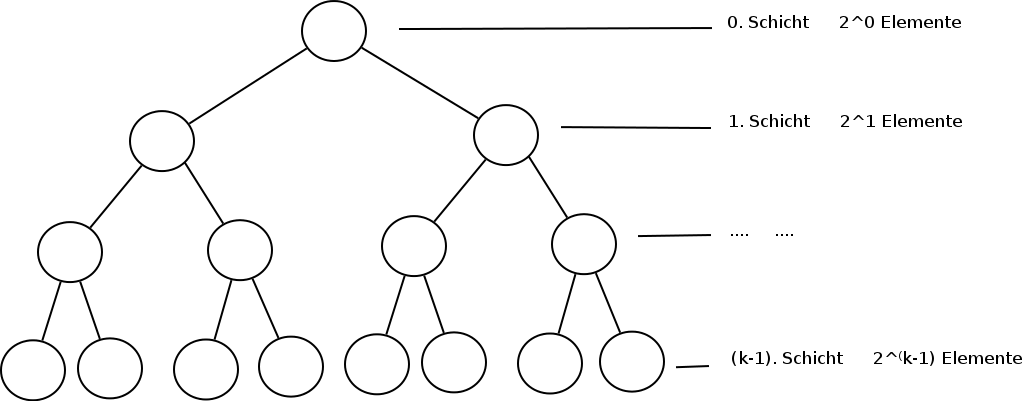
\includegraphics[width=0.8\linewidth]{2/Grafik/img1.png}
\end{figure}

$n :=$ Zahl der Elemente\\
$k :=$ Zahl der Schichten

\subsection{Zusammenhang von n und k}
\begin{flalign*}
&n=\sum_{i=0}^{k-1} 2^i = 2^k -1 &
\end{flalign*}


\begin{mdframed}
\paragraph{Merke: Geometrische Reihe}
\begin{flalign*}
&\sum_{i=0}^{k-1} x^i = \frac{1-x^k}{1-x}~~~\text{mit}~x\not= 1 &
\end{flalign*}\\

\end{mdframed}


\newpage

\subsection{Analyse Heapaufbau}
\begin{flalign*}
&\sum_{l=0}^{k-1} 2^l (k-1-l) &\\
\\
&2^l~~~~~~~~~~~:= ~\text{Anzahl Knoten auf Level l}&\\
&(k-1-l) := ~\text{Leveldifferenz zwischen l und der Blattebene}&\\
\\
&\sum_{l=0}^{k-1} (k-1-l) \cdot 2^l = \sum_{l=0}^{k-1} (k-1) \cdot 2^l - \sum_{l=0}^{k-1}l \cdot 2^l  = (k-1)(2^k-1)-2 \sum_{l=1}^{k-1}l2^{l-1}&
\end{flalign*}\\
%
\begin{mdframed}
\paragraph{Nebenrechnung}
\begin{flalign*}
&\sum_{i=1}^{k-1} i \cdot x^{i-1} = \frac{d}{dx} \left(\sum_{i=0}^{k-1} x^i \right) = \frac{d}{dx} \left(\frac{x^k-1}{x-1} \right) &\\
& = \frac{kx^{k-1}(x-1)-(x^k-1)}{(x-1)^2} &\\
&\text{mit}~x=2~\text{folgt:}~~~~~k\cdot 2^{k-1}-2^k+1&
\end{flalign*}\\
\end{mdframed}


\begin{flalign*}
&=(k-1)(2^k-1)-k2^k+2^{k+1}-2 &\\
&=k2^k-2^k-k+1-k2^k+2^{k+1}-2&\\
&=-2^k-k-1+2^{k+1} \leq 2^{k+1} \approx 2 \cdot n&\\
\\
&\Rightarrow \text{Heapaufbau in lineare Zeit}&
\end{flalign*}\\


\subsection{Sortierphase}
\paragraph{1. Versuch} $n \cdot k~~~~$ mit $n= 2^k-1 \Leftrightarrow k = \log_2(n+1) \approx n \cdot \log_2(n)$
\paragraph{2. Versuch (mit Verkleinerung der Liste)} 
\begin{flalign*}
&\sum_{l=0}^{k-1} 2^l \cdot l = 2 \sum_{l=1}^{k-1} l \cdot 2^{l-1} = 2 \cdot (k \cdot 2^{k-1} - 2^k+1) \geq k \cdot 2^{k-1} \approx n \cdot \log_2(n)&
\end{flalign*}\\


\pagebreak

\subsection{Fazit}
\paragraph{Laufzeit} $c \cdot n \cdot \log_2(n)~~~~$ wobei $c \in \mathbb{R}$

\paragraph{Vergleich} \textcolor{Red}{Bubblesort} $\leftrightarrow$ \textcolor{Green}{Heapsort}
\begin{center}
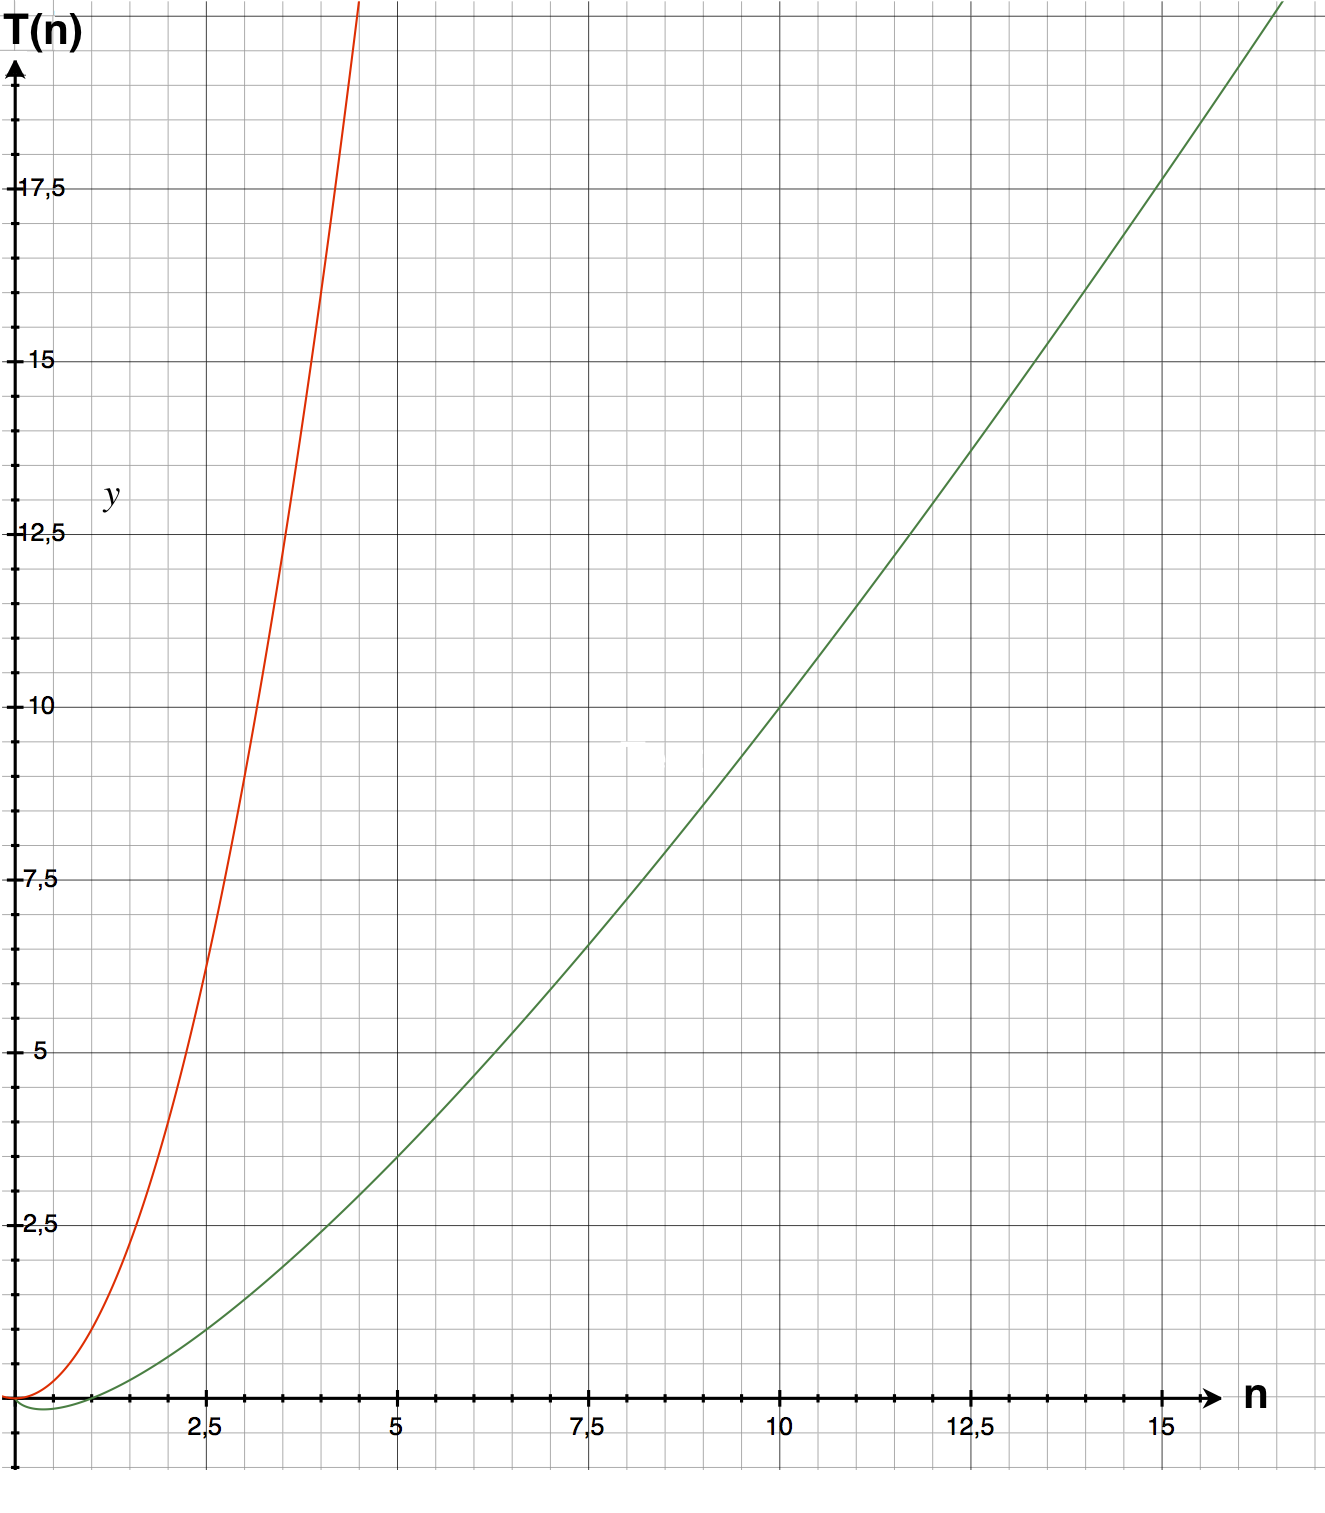
\includegraphics[width=0.8\linewidth]{2/Grafik/Bubble_rot_heap_gruen.png}
\end{center}
